\chapter{Literatures}

\section{Fission related}

%%%%%%%%%%%%%%%%%%%%%%%%%%%%%%%%%%%%%%%%%%%%%%%%%%%%%%%%%%%%%
\noindent\rule[0.25\baselineskip]{\textwidth}{2pt}
\noindent \textcolor{blue}{\textbf{[1] H. Tao, J. Zhao, Z.P. Li, T. Niksi{\'c}, and D. Vretenar, Microscopic study of induced fission dynamics of $\prescript{226}{}{\rm \mathbf{Th}}$ with convariant energy density functionals, Phy.Rev.C 96, 024319(2017)}}
\begin{itemize}[leftmargin=10pt]
    \item \textbf{NOTES}
        \begin{enumerate}[leftmargin=10pt]
            \item Main Idea \newline
                \begin{tikzpicture}[node distance=10pt]
                    \node[draw, text width=5cm]      (start)  {PES(quadrupole $\beta_2$, octupole $\beta_3$,potentia $V$, and mass parameters $B_{22}$, $B_{23}$, $B_{33}$)};
                    \node[draw, left=70pt of start]  (step1)  {PC-PK1 + $\delta$-force};
                    \node[draw, below=30pt of start] (step2)  {Fission Dynamics(GCM+GOA)};
                    \node[draw, right=70pt of step2] (step3)  {Fission Yields};

                    \draw[<-]  (start) -- node[above] {\footnotesize{Calculate and get}} (step1);
                    \draw[->] (start) -- node[right] {\footnotesize{as an input}} (step2);
                    \draw[->]  (step2) -- node[above] {\footnotesize{Calculate and get}} (step3);
                \end{tikzpicture}
                
            \item Coordinate   \newline
                $\hat{Q}_k$ denotes the expectation value of the mass quadrupole and the octupole operators
                \begin{equation}
                    \hat{Q}_2 = 2z^2 - r_{\bot}^2 \quad \text{and} \quad \hat{Q}_3 = 2z^3 - 3zr_{\bot}^2    \label{b1}
                \end{equation}
                The corresponding deformation parameters $\beta_2$ and $\beta_3$ can be determined from the following relations:
                \begin{equation}
                    \begin{aligned}
                        \beta_2 = \frac{\sqrt{5\pi}}{3AR_0^2}\langle \hat{Q}_2 \rangle,   \quad
                        \beta_3 = \frac{\sqrt{7\pi}}{3AR_0^3}\langle \hat{Q}_3 \rangle  \label{b2}  
                    \end{aligned}
                \end{equation}
                with $R_0 = r_0 A^{1/3}$ and $r_0 = 1.2{\rm fm}$.\newline
                \textbf{Example -- Phy.Rev.C 93, 054611 (2016)}\\
                The quadrupole and octupole moments in this article is 
                \begin{equation}
                    \hat{Q}_{20} = 2z^2 - r_{\bot}^2 \quad \text{and} \quad \hat{Q}_{30} = \sqrt{\frac{7}{4\pi}}(z^3 - zr_{\bot}^2) \label{b3}
                \end{equation}
                the unit for $\hat{Q}_{20}$ is $barn(b)$, we have $1b = 100fm^2$, and unit for $\hat{Q}_{30}$ is $b^{3/2}$, the definition is different from \eqref{b1}, according to \eqref{b1}-\eqref{b3}, we have the transformational relation 
                \begin{equation}
                    \begin{aligned}
                        \beta_2 = \frac{\sqrt{5\pi}}{3AR_0^2}\langle \hat{Q}_{20} \rangle,   \quad
                        \beta_3 = \frac{4\pi}{3AR_0^3}\langle \hat{Q}_{30} \rangle
                    \end{aligned}
                \end{equation}

            \item Strengths parameters of $\delta$-force    \\
                Using a five-point formula to cacluate the pairing gap parameters:
                \begin{equation}
                    \Delta_{q}^{(5)} (N_0) = -\frac{\pi_{N_0}}{8} \left[ E(N_0 + 2) - 4E(N_0 + 1) + 6E(N_0) - 4E(N_0 - 1) + E(N_0 -2) \right]
                \end{equation}
                where $\pi_{N_0} = (-1)^{N_0}$, $N_0$ reprecent numbers of protons or neutrons in the nuclei that we need to calculate.
            \item Neck Operator     \\
                \begin{equation}
                    \hat{Q}_N = exp\left[ \frac{-(z-z_n)^2}{a_N^2} \right]
                \end{equation}
                where $a_N = 1$fm and $z_N$ is the position of the neck[56].
            \item Total Kinetic Energy  \\
                \begin{equation}
                    E_{TKE} = \frac{e^2 Z_H Z_L}{d_{ch}}
                \end{equation}
                where $e$ is the proton charge, $Z_H(Z_L)$ is the charge of the heavy(light) fragment, $d_{ch}$ is the distance between fragment centers of charge at scission.
        \end{enumerate}

    \item \textbf{Result and Discussion}
        \begin{enumerate}[leftmargin=10pt]
            \item Pairing Strength    \newline
                The general topography of the PESs does not change significantly as pairing increases, the barriers are reduced considerably.   \newline
                %\noindent 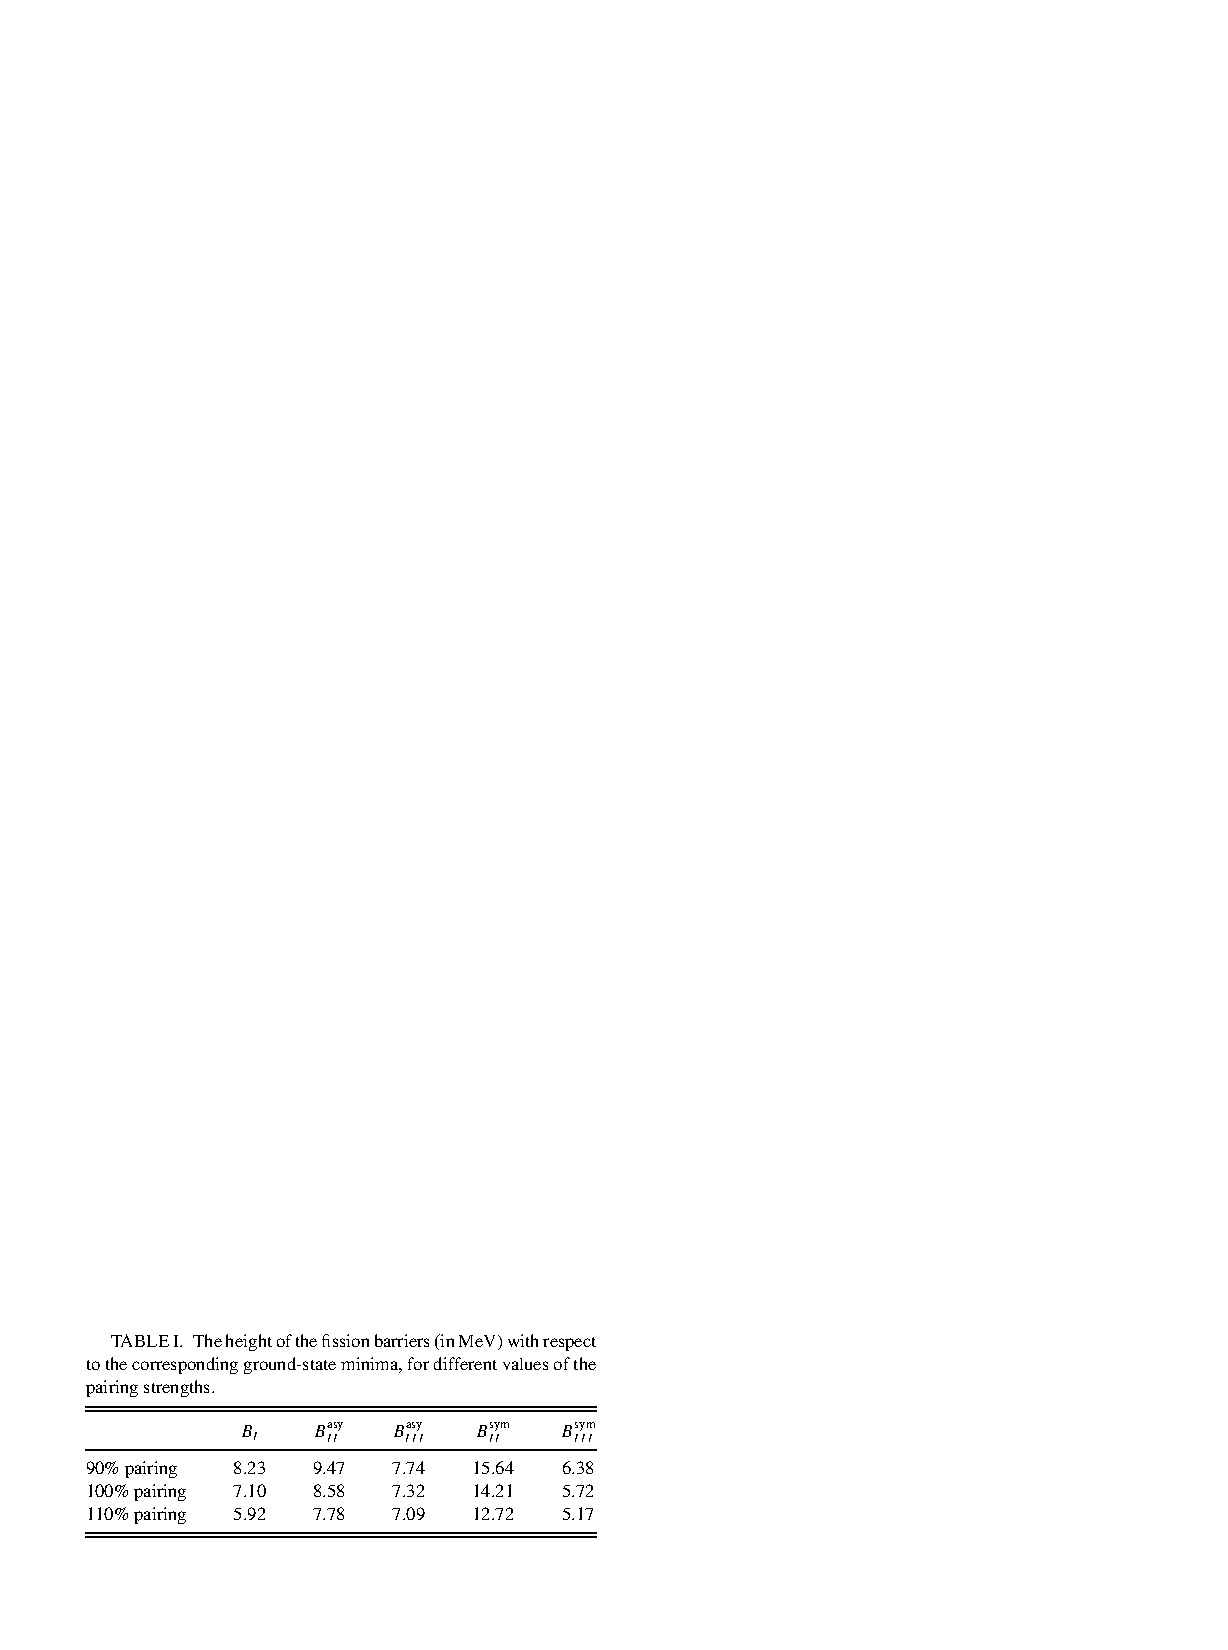
\includegraphics[width=7cm]{figure/literatures/reference-1_2.pdf} \newline
                As pairing correlations increase, the collective masses are reduced and the shell oscillations are also reduced. And the pattern of the scission line does not change significantly with the varience of the pairing strength.  \newline
                The pairing strength influence the fission yields significantly due to the reduction of the ridge between asymmetric and symmetric fission when increasing the pairing strength.
            \item Excitation Energy \newline
                With the increase in energy, the current can more directly enter the symmetric valle and, consequently, the asymmetric peaks are lowered while the symmetric peak gradually bcomes wider.
        \end{enumerate}
\end{itemize}

%%%%%%%%%%%%%%%%%%%%%%%%%%%%%%%%%%%%%%%%%%%%%%%%%%%%%%%%%%%%%%
\vspace{8pt}
\noindent\rule[0.25\baselineskip]{\textwidth}{2pt}
\noindent \textcolor{blue}{\textbf{[2] D. Regnier, N. Dubray and N. Schunck, From asymmetric to symmetric fission in the fermium isotopes within the time-dependent generator-coordinate-method formalism, Phy.Rev.C 99, 024611(2019)}}
\begin{itemize}[leftmargin=10pt]
    \item \textbf{Words}
    \begin{enumerate}[leftmargin=10pt]
        \item  \textcolor{red}{In heavy and superheavy nuclei, a difference of only a few neutrons is sufficient to change the dominant fission mode.}
        \item More recently, studies of static deformation properties of fermium isotopes were also performed within a self-consistent meanfield framework based on Gogny, Skyrme, and covariant energy density functionals (EDFs) [17-22]. All these papers emphasized the multimodal character of the fission of fermium isotopes near A = 256 and highlighted the presence of three major modes: symmetric compact, symmetric elongated, and asymmetric.
        \item In the TDGCM+GOA picture, the presence of valleys in the potential energy landscape favors the diffusion of the collective wave packet toward specific sets of configurations at scission.
        \item At $Q_{20}=140{\rm b}$, symmetric configurations are largely favored energetically in all three isotopes. 
    \end{enumerate}

    \vspace{5pt}
    \item \textbf{Note}
        \begin{enumerate}[leftmargin=10pt]
            \item Main Idea \newline
                \begin{tikzpicture}[node distance=10pt]
                    \node[draw]                      (start)  {PES};
                    \node[draw, left=70pt of start, text width=4.5cm]  (step1)  {Gogny effective interaction \\ (in a two-center HO basis)};
                    \node[draw, below=30pt of start] (step2)  {Fission Dynamics(GCM+GOA)};
                    \node[draw, right=70pt of step2] (step3)  {Fission Yields};

                    \draw[<-]  (start) -- node[above] {\footnotesize{Calculate and get}} (step1);
                    \draw[->] (start) -- node[right] {\footnotesize{as an input}} (step2);
                    \draw[->]  (step2) -- node[above] {\footnotesize{Calculate and get}} (step3);
                \end{tikzpicture}
            \item Fission Mode  \newline
                symmetric compact fission mode[19, 21], symmetric elongated fission mode.   \newline
                The rapid decreasing of potential around $Q_{20} \simeq 220b$ is correspods to the symmetric fission mode.
            \item PES   \newline
                The potential ridge is indeed quite pronounced for $\prescript{258}{}{\rm Fm}$ but progressively disappears as we go toward the lighter isotopes.
            \item Fission Fragments Distributions   \newline
                Taking into account the \underline{neutron evaporation} would shift our predictoins by a few units toward lighter masses as well as bring additional structure and asymmetry between the light and heavy peaks.   \newline
                A second important effect that also impacts the comparison with experiment is the \underline{initial energy} of the fissioning system.
        \end{enumerate}
    \item My confusion
        \begin{enumerate}[leftmargin=10pt]
            \item \textcolor{red}{What is disentanglement of the fragment?}
        \end{enumerate}
    \item \textbf{\textcolor{red}{My Thinking}} \newline
        It may be important to analysis the potential variety along the $Q_{30}$ around the scission point when keeping $Q_{20}$ a constant(\textcolor{cyan}{see ${\rm \uppercase\expandafter{\romannumeral3}.A.2}$}).
\end{itemize}

%%%%%%%%%%%%%%%%%%%%%%%%%%%%%%%%%%%%%%%%%%%%%%%%%%%%%%%%%%%%%%
\vspace{8pt}
\noindent\rule[0.25\baselineskip]{\textwidth}{2pt}
\noindent \textcolor{blue}{\textbf{[3] Guillaume Scamps${}^*$, C{\' e}dric Simenel${}^{\dag}$, Denis Lacroix${}^{\ddag}$, Superfluid dynamics of $\prescript{258}{}{\rm Fm}$ fission, Phy.Rev.C 92, 011602(R)(2015)}}
\begin{itemize}[leftmargin=10pt]
    \item \textbf{Words}
        \begin{enumerate}[leftmargin=10pt]
            \item Indeed, magic fragments are difficult to excite and deform and, thus, fission occurs faster \textcolor{red}{as less dissipation is involved}, leading to a larger TKE.
        \end{enumerate}
        
\end{itemize}

%%%%%%%%%%%%%%%%%%%%%%%%%%%%%%%%%%%%%%%%%%%%%%%%%%%%%%%%%%%%%%
\vspace{8pt}
\noindent\rule[0.25\baselineskip]{\textwidth}{2pt}
\noindent \textcolor{blue}{\textbf{[4] W. Younes and D. Gogny, Nuclear Scission and Quantum Localization, Phys.R}}
\begin{itemize}[leftmargin=10pt]
    \item Essential Words
    \begin{enumerate}[leftmargin=10pt]
        \item The disentanglement of the fragment wave functions is essential to the quantum-mechanical definition of scission and the calculation of physical observables.
        \item Scission implies a separation of the nucleus into independent fragments, \textcolor{blue}{while the Pauli exclusion principle introduces a persistent correlation between the fragments, no matter how far apart they are.}
    \end{enumerate}

    \vspace{5pt}
    \item Some elegant Words
        \begin{enumerate}[leftmargin=10pt]
            \item 
        \end{enumerate}
    
    \vspace{5pt}
    \item My confusion
        \begin{enumerate}[leftmargin=10pt]
            \item \textcolor{red}{What is disentanglement of the fragment wave functions?}(reference [6])
            \item \textcolor{red}{What is the definition of the neck size?}(reference[9])
            \item \textcolor{red}{Where is the "tails"?}(reference[9])
            \item \textcolor{red}{Bogoliubov vacuum is only defined up to a unitary transformation of the qp destruction operators.}(Why?)
        \end{enumerate}
\end{itemize}

%%%%%%%%%%%%%%%%%%%%%%%%%%%%%%%%%%%%%%%%%%%%%%%%%%%%%%%%%%%%%%
\vspace{8pt}
\noindent\rule[0.25\baselineskip]{\textwidth}{2pt}
\noindent \textcolor{blue}{\textbf{[5] W. Younes and D. Gogny, Microscopic calculation of $\sideset{^{240}}{}{\mathop{\mathbf{Pu}}}$ scission with a finite-range effective force, Phy.Rev.C 80, 054313(2009)}}
\begin{itemize}[leftmargin=10pt]
    \item some useful points
    \begin{enumerate}[leftmargin=10pt]
        \item 
    \end{enumerate}
\end{itemize}

%%%%%%%%%%%%%%%%%%%%%%%%%%%%%%%%%%%%%%%%%%%%%%%%%%%%%%%%%%%%%%
\vspace{8pt}
\noindent\rule[0.25\baselineskip]{\textwidth}{2pt}
\noindent \textcolor{blue}{\textbf{[6] A. Zdeb, A. Dobrowolski and M. Warda, Fission dynamics of $^{252}Cf$, Phy.Rev.C 95, 054608(2017)}}
\begin{itemize}[leftmargin=10pt]
    \item  \textbf{Words}
    \begin{enumerate}[leftmargin=10pt]
        \item Calculat the PES by HFB model with the D1S Gogny-type interactions.
        \item Calculat the dynamic of fission within TDGCM+GOA formalism.
    \end{enumerate}
    \item Some points
    \begin{enumerate}[leftmargin=10pt]
        \item It has been shown that minimization of action integral with the nonperturbative mass parameters modifies the fission trajectory in the barrier region. The penetration probability is higher in comparison to that resulting from dynamic calculations within perturbative inertias.
    \end{enumerate}
\end{itemize}

%%%%%%%%%%%%%%%%%%%%%%%%%%%%%%%%%%%%%%%%%%%%%%%%%%%%%%%%%%%%%%
\vspace{8pt}
\noindent\rule[0.25\baselineskip]{\textwidth}{2pt}
\noindent \textcolor{blue}{\textbf{[7] J${\rm o\mkern-8.5mu/}$rgen Randrup and Ramona Vogt, Generation of Fragment Angular Momentum in Fission, Phy.Rev.L 127, 062502(2021)}}
\begin{itemize}[leftmargin=10pt]
    \item \textbf{Question}
    \item What \newline
        \underline{Binary character} prior to scission[12] \newline
        \underline{Six dinuclear rotational modes:} wriggling and bending(double degenerate), twisting and tilting[13,14]\newline
        What is the meaning of the setence \textcolor{red}{"In particula, expressions were derived for associated mobility coefficients which ... so it remains in local equilibrium."}\newline
        What is the \underline{statistical fluctuations} in angular momentum.
    \item \textbf{Words}
    \begin{enumerate}[leftmargin=10pt]
        \item 
    \end{enumerate}
    \begin{enumerate}[leftmargin=10pt]
        \item 
    \end{enumerate}
    \item \textbf{Some points}
    \begin{enumerate}[leftmargin=10pt]
        \item 
    \end{enumerate}
\end{itemize}

%%%%%%%%%%%%%%%%%%%%%%%%%%%%%%%%%%%%%%%%%%%%%%%%%%%%%%%%%%%%%%
\vspace{8pt}
\noindent\rule[0.25\baselineskip]{\textwidth}{2pt}
        \noindent \textcolor{blue}{\textbf{[8] N. Schunck and L.M. Robledo, Microscopic theory of nuclear fission: a review, Rep. Prog. Phys. 79(2016), 116301}}
\begin{itemize}[leftmargin=10pt]
    \item \textbf{Abstract}
        \begin{enumerate}[leftmargin=10pt]
            \item In \underline{spotaneous fission}, the half-lives are the main observables and quantum tunnelling the essential concept; in \underline{induced fission}, the focus is on fragment properties and explicitly time-dependent approaches are often invoked.
            \item Overall, the cornerstone of the density functional theory approch to fission is the energy density functional formalism.
        \end{enumerate}
    \item \textbf{Introduction}
        \begin{enumerate}[leftmargin=10pt]
            \item The nuclear 'fissility' parameter:
                \begin{equation}
                    x \approx \frac{Z^2}{50.88A(1-\eta I^2 )}
                \end{equation}
                where $I = (N - Z)/A$ and $\eta = 1.7826$ [6-8]. In the liquid drop model, the fissility is related to the ratio between the Coulomb and surface energy of the drop. for values of $x > 1$, the drop is unstabel against fission, and nulcear fission can then occur spontaneously.
            \item Nuclear fission also plays an important role in the formation of elements in the rapid neutron capture process(r-process) of nucleosynthesis in stellar environments.
            \item Because of the \underline{strong nuclear binding}, the energy released during fission is very large (compared to other energy production sources), typically of the order of 200 MeV per fission event. Most of it is kinetic energy of the fission fragments while about $10\sim 20\%$ of it is excitation energy. 
        \end{enumerate}
    \item \textbf{Potential energy surfaces} \newline
        The \textcolor{red}{cornerstone} of the implementation of the adiabatic approximation in fission theory is the definition of a \textcolor{red}{potential energy surface(PES)} in an arbitrary collective space. 
        \begin{enumerate}[leftmargin=10pt]
            \item \textcolor{cyan}{\underline{The macroscopic-microscopic approach}}\newline
                \underline{Main Idea:} The MM approach consists in viewing the nucleus as a finite chunk of nulcear matter, the energy of which is parametrized as a function of the charge, mass and deformations $\bm{q}$ of the nucleus.\newline
                \underline{Total Energy:} (i)$E_{mac}$ is the macroscopic energy obtained by a deformed liquid drop or droplet formula, represets bulk nuclear properties;(ii) a shell correction $E_{shell}$, accounts for the distribution of single particle levels in the average nuclear potential and thus has a one-body origin;(iii) a pairing correction $E_{pair}$, which has a two-body origin. The formation of the total energy is
                \begin{equation}
                    E(\bm{q}) = E_{mac}(\bm{q}) + E_{shell}(\bm{q}) + E_{pair}(\bm{q})
                \end{equation}
                In MM approach, we \textcolor{red}{first} formula a formulation to describe the nuclear shape, \textcolor{red}{then} we introduce some microscopic quantum corrections(just like shell, pairing correlation correction) in the macroscopic energy. 
                \begin{enumerate}
                    \item Parametrization of the nuclear surface \newline
                        The simplest and most common parametrization is based on the multipole expansion of the nuclear radius[56]:
                        \begin{equation}
                            R(\theta, \varphi)=R_{0} c(\alpha)\left[1+\sum_{\lambda \geqslant 2} \sum_{\mu=-\lambda}^{+\lambda} \alpha_{\lambda \mu} Y_{\lambda \mu}(\theta, \varphi)\right]
                        \end{equation}
                        where $R_0 = r_0 A^{1/3}$ is a parametrization of the nuclear radius for a spherical nulceus of mass $A(r_0 \approx 1.2 {\rm fm})$; $c(\alpha)$ is a factor accounting for the conservation of nuclear volume with deformation; the $\alpha_{\lambda\mu}$ are the deformation parameters; $Y_{\lambda\mu}(\theta,\phi)$ are the usual spherical harmonics.
                \end{enumerate}
        \end{enumerate}
    
\end{itemize}
%%%%%%%%%%%%%%%%%%%%%%%%%%%%%%%%%%%%%%%%%%%%%%%%%%%%%%%%%%%%%%
\vspace{8pt}
\noindent\rule[0.25\baselineskip]{\textwidth}{2pt}
        \noindent \textcolor{blue}{\textbf{[9] D. Regnier,${}^{1,*}$ N. Dubray,${}^{1,\dagger}$ N. Schunck, ${}^{2,\ddagger}$ and M. Verrière, Fission fragment charge and mass distribution in $\sideset{^{239}}{}{\mathop{\mathbf{Pu(n,f)}}}$ in the adiabatic nuclear energy density functional theory, Phy. Rev. C 93, 054611(2016)}}
\begin{itemize}[leftmargin=10pt]
    \item
\end{itemize}
%%%%%%%%%%%%%%%%%%%%%%%%%%%%%%%%%%%%%%%%%%%%%%%%%%%%%%%%%%%%%%
%%%%%%%%%%%%%%%%%%%%%%%%%%%%%%%%%%%%%%%%%%%%%%%%%%%%%%%%%%%%%%
\section{Density Functional}

\noindent\rule[0.25\baselineskip]{\textwidth}{2pt}
\noindent \textcolor{blue}{\textbf{[1] P.W. Zhao, Z.P. Li, J.M. Yao and J. Meng, New parametrization for the nuclear convariant energy density functional with a point-coupling interaction, Phy.Rev.C 82, 054319(2010)}}
\begin{itemize}[leftmargin=10pt]
    \item The main result of the theory
    \begin{enumerate}[leftmargin=10pt]
        \item The total energy for the nuclear system
        \begin{equation}
            E_{\mathrm{tot}}=E_{\mathrm{DF}}\left[\boldsymbol{\tau}, \rho_{S}, j_{i}^{\mu}, A_{\mu}\right]+ E_{\text {pair }}\left[\kappa, \kappa^{*}\right] + E_{\mathrm{c} . \mathrm{m} .}^{\mathrm{mic}}
        \end{equation}
        where the \textcolor{red}{center-of-mass(c.m.) correction energy } is
        \begin{equation}
            E_{\mathrm{c} . \mathrm{m} .}^{\mathrm{mic}} = -\frac{1}{2mA}\langle \hat{\boldsymbol{P}}^2_{c.m.} \rangle
        \end{equation}

    \end{enumerate}
\end{itemize}